\chapter{Auswertung}
Im letzten Teil dieser Arbeit wird das Huff-Modell und dessen Umsetzung im Prototypen ausgewertet.\\
Was sind die Anwendungsfälle des Huff-Modells?
Wozu kann der Prototyp verwendet werden?
Ist der Prototyp performant?
Ist das Huff-Modell eine gute Wahl für einen Algorithmus der Filialplanung und Standortanalyse?
Wo stößt das Modell an seine Grenzen?
Was kann verbessert, erweitert oder ersetzt werden?

Unter Anderem diesen Fragen wird mit Ausblick auf die Zukunft kritisch Antwort gegeben bevor ein finales Fazit gezogen wird.

\section{Bewertung}
Bei der Bewertung des Prototypen muss einerseits die Umsetzung des Huff-Modells in einer Webkarte mit modernen Technologien und andererseits das Modell selber bewertet werden.
Hierzu werden zunächst Anwendungsfälle des Modells beschrieben, die Verwendung des Prototypen unter Einbeziehung der Performance für diese erklärt und Verbesserungen und Erweiterungen vorgestellt.
Danach wird das Modell selber in Frage gestellt und mögliche Alternativen oder Erweiterungen vorgestellt.

Obwohl das Huff-Modell kein neues Phänomen ist und schon mehrere Jahrzehnte alt ist, hat es sich als verlässlich erwiesen und findet nach wie vor Gebrauch.
Die liegt vor Allem an der einfachen und schnellen Verwendung. 
Bereits mit wenig Informationen können simple Prognosen zu Besucherwahrscheinlichkeit erstellt werden.\\
Zu den Hauptanwendungsfällen zählen:

\begin{itemize}
	\item Filialplanung
	\item Expansionsplanung
	\item Verteilgebietsplanung
	\item Kundenansprache
\end{itemize}

Die Filialplanung und Expansionsplanung sowie die Verteilgebietsplanung und die Kundenansprache sind ähnlich zu betrachten, da sie sich nur geringfügig Unterscheiden.\\
Der Prototyp kann alle aufgelisteten Fälle grundlegend abdecken,könnte aber aber bei gezielten Erweiterungen eine noch bessere Unterstützung für die spezifischen Anforderungen bieten.
So lassen sich Besuchswahrscheinlichkeiten in bestehendem Netz sowie mit neuen Filialen berechnen und vergleichen.
Potenzielle neue Standorte können dem bestehenden Netz hinzugefügt werden und deren Auswirkung auf Wahrscheinlichkeiten und Umsatz werden direkt visuell und numerisch sichtbar, was bei direktem Vergleich eine Erstellung einer Reihenfolge anhand von Umsatzgewinn oder -verlust und Marktanteil der potenziellen neuen Standorte erlaubt.\\
Hierzu wäre eine Erweiterung hinsichtlich direkter Gegenüberstellung der potenziellen Standorte in Form einer Tabelle oder Ähnlichem denkbar. 
Im Prototyp lassen sich zwar beliebig viele neue Filialen setzen, jedoch gibt es keine Möglichkeit die gesetzten Filialen und deren Einfluss auf Wahrscheinlichkeiten und Marktanteil zu vergleichen.

Ebenso kann sehr leicht ein Verteilgebiet für Handzettel (Werbung) abgegrenzt werden, dass sich auch wirklich nur an Kunden richtet, die wahrscheinlich in der Filiale einlaufen würden.
Außerdem sind aus den Gebieten des Verteilgebiets erste Informationen zu Kaufkraft, Einwohneranzahl und Ausgaben ersichtlich, welches eine persönlichere Ansprache der Kunden zulässt, die auf demografischen Analysen beruht.\\
Eine sinnvolle Erweiterung für die Verteilgebietserstellung wäre die Gruppierung mehrerer Gebiete zu einem neuen Verteilgebiet in einem neuen Layer.
Das neue Gebiet könnte dann eine eigene Farbe erhalten und nach Bedarf ein- und ausgeblendet werden oder in der Z-Ebene nach oben oder unten verschoben werden.
Für das neue Gebiet können dann die Daten der eingeschlossenen Gebiete summiert werden und für das potenzielle Verteilgebiet angezeigt werden.

Die Berechnung des Modells ist bereits angemessen performant mit initialer Lade- und Renderzeit von unter 1 Sekunde für die Gebiete und Filialen sowie Berechnungs- und Rerenderzeit der Gebiete von ebenfalls unter 1 Sekunde.
Durch Optimierung beim Laden und Rendern durch zum Beispiel explizite Nutzung von Cache-Objekten für Features und Styles oder Überarbeitung des Codes für die Berechnung des Modells, könnte hier eventuell noch ein wenig mehr Performance optimiert werden.

Der Prototyp kann das Huff-Modell sehr gut darstellen und bietet echten Mehrwert in Prozessen des Geomarketings.
Dennoch hat das Modell auch einige Schwächen oder Ungenauigkeiten, wie bereits im Artikel "Application of network Huff model for commercial network planning at suburban – Taking Wujin district, Changzhou as a case" von Haozhi Pan,Yongfu Li und Anrong Dang beschrieben \footcite{pan_application_2013}.
Die Autoren stellen vor Allem die Bestimmung der Parameter $\alpha$ und $\beta$ sowie die Berechnung der Distanzvariable D als problematisch hervor.
Während es für die Bestimmung der Parameter meist an regionalen Marktdaten mangelt oder eine Regressionsanalyse mit Linearisierung nur schwer durchzuführen ist, so gibt es schlichtweg mehrere Möglichkeiten die Distanz zwischen Filiale und Kunde zu berechnen.
Die Distanz kann euklidisch dargestellt werden oder über die Netzwerkdistanz oder - zeit (Fahrzeitzone in Meter oder Minuten) wobei alle drei zu verschiedenen Ergebnissen des Modell führen.
Ebenso finden sich direkt im Prototypen einige Schwächen wieder.\\
So lassen sich Filialen finden, bei denen die Berechnung zu einem ungenauen Ergebnis, wie in Abbildung \ref{img:innacc_store} zu sehen, führt.
In der Abbildung ist klar zu erkennen, dass das Gebiet in welchem sich die Filiale befindet selbst nicht die höchste Besuchswahrscheinlichkeit hat.
Diese Ungenauigkeit lässt sich auf die Berechnung des Mittelpunkts des Gebiets zurückführen, so ist die Filiale näher am Mittelpunkt des Nachbargebiets als am Mittelpunkt des eigenen Gebiets gelegen, was zu einer höheren Besuchswahrscheinlichkeit des Nachbargebiets führt.\\
Dieses Problem lässt sich relativ einfach mit der Verwendung von kleineren Gebieten eindämmen.
Jedoch ist die ideale Lösung mit der Verwendung von Punkten pro Haushalten nicht wirklich umsetzbar, da die Datenmenge um ein Vielfaches größer wäre und die Berechnung zu viel Ressourcen benötigen oder zu lange dauern würde.

\begin{figure}[H]
	\makebox[\textwidth][c]{
		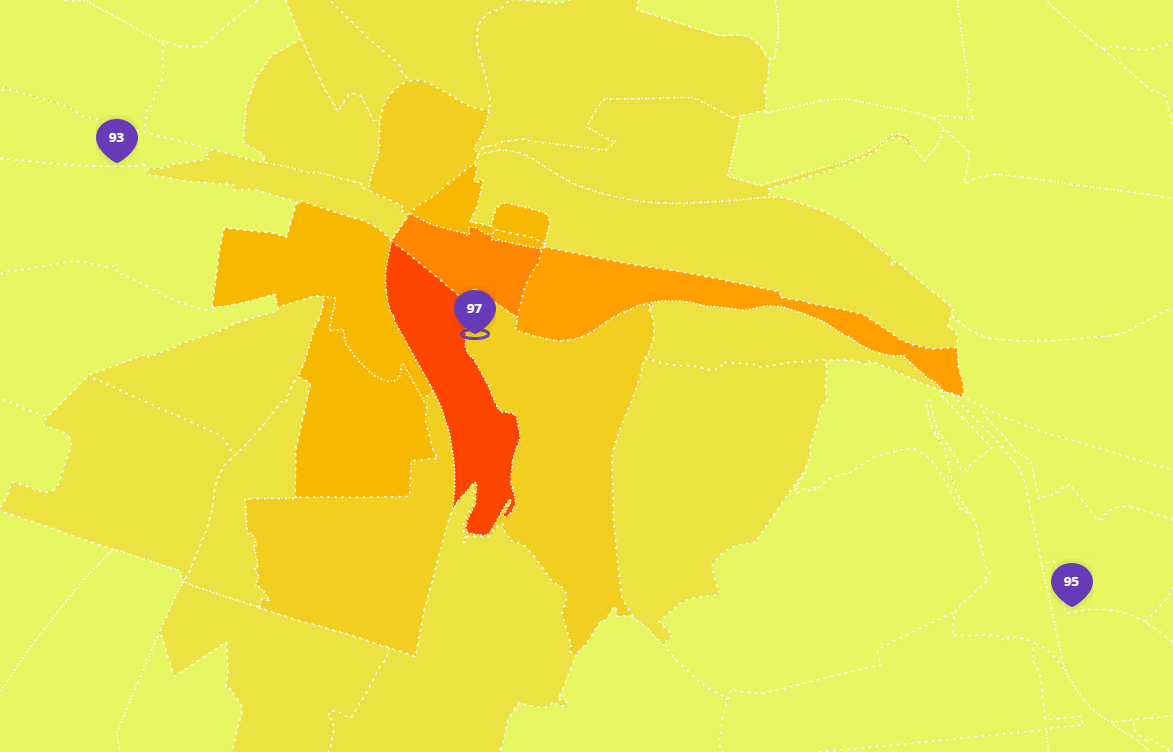
\includegraphics[scale=0.4]{resources/images/ungenaue_filiale.png}}
	\caption{Bildschirmausschnitt des Prototypen mit ungenauer Berechnung}
	\label{img:innacc_store}
\end{figure}

Weiterführend können zwar die Attraktivität und Distanz nahezu beliebig genau Errechnet werden, jedoch werden auch nur genau diesen beiden Variablen in die Berechnung einbezogen.
Aufgrund dieser Einschränkung und vor Allem den bereits aufgeführten Problemen in Bezug auf die Bestimmung der Parameter $\alpha$ und $\beta$ war das Huff-Modell im Laufe der Jahre bereits mehrfach Kern wissenschaftlicher Arbeiten, die sich mit der Validierung und Verbesserung des Modells beschäftigten.\\
So entstand 1974 das Multiplicative Competitive Interaction Modell (kurz MCI-Modell), welches genau diese Probleme behandelt \footcite{nakanishi_parameter_1974}.  

\section{Fazit/ Ausblick}
Das Huff-Modell als Grundlage der algorithmischen Berechnung in dem Prozess einer Filialplanung erweist sich als einfach zu verstehendes, schnelles und nützliches Werkzeug, um mit relativ wenig Marktdaten bereits eindeutige und aussagekräftige Informationen über mögliche neue Standorte einer Filiale zu erhalten.\\
Im Prototypen wurden die verfügbaren Marktdaten um lediglich ein paar wenige Attribute ergänzt, um eine realistische Abbildung eines Filialnetzes innerhalb Berlins zu generieren. 
Die Parameter der Berechnung lassen sich hierbei einfach fast beliebig Erweitern, so können in die Berechnung der Attraktivität deutlich mehr Attribute einer Filiale oder des Umfelds einfließen.
Denkbar wären zum Beispiel die Ergänzung von Informationen über umliegende Sehenswürdigkeiten (engl. Point of interest), die Eingliederung der Filiale in ein Einkaufszentrum, Markenstärke einer Filialkette oder tatsächliches Sortiment, welche alle Einfluss auf die Attraktivität einer Filiale nehmen.\\
Ebenso kann die Berechnung der Distanz auf komplexeren Grundlagen wie zum Beispiel der Fahrzeit mit dem Auto, den öffentlichen Verkehrsmitteln oder dem Fahrrad basieren.\\
Bereits im Kapitel\ref{subsec:gravitationmodel} Gravitationsmodell erwähnt, sollten die Parameter $\alpha$ und $\beta$ empirisch bestimmt werden.
Der Komplexität der Erhebung der Parameter ist hierbei keine Grenze gesetzt. 
Kundenbefragungen, amtliche Statistiken oder Meinungsbilder aus der freien Wirtschaft können hier als Grundlage dienen.\\
Für die Anwendung in echten Szenarien der freien Wirtschaft sollten also unbedingt eine verfeinerte Kalibrierung der Berechnung anhand eigener Daten erfolgen, damit der Prototyp zum vollen Potenzial verwendet wird.

Als Komponente eines größeren, komplexeren GIS, würde der Prototyp einzigartige, ergänzende Features bieten, die die Prozesse innerhalb der Standortanalyse und Filialplanung deutlich vereinfachen.\\